\documentclass[landscape,a0paper,fontscale=0.25]{tikzposter}

% Packages
\usepackage{amsmath}
\usepackage{amssymb}
\usepackage{graphicx}
\usepackage{enumitem}
\usepackage{url}
\usepackage{tikz}
\usetikzlibrary{shapes,arrows,positioning}

% Color theme - Academic
\definecolorstyle{AcademicStyle}{
    \definecolor{colorOne}{RGB}{26,54,93}      % Navy blue
    \definecolor{colorTwo}{RGB}{39,103,73}     % Forest green
    \definecolor{colorThree}{RGB}{247,250,252} % Light gray
}{
    \colorlet{backgroundcolor}{white}
    \colorlet{framecolor}{colorOne}
    \colorlet{titlefgcolor}{white}
    \colorlet{titlebgcolor}{colorOne}
    \colorlet{blocktitlebgcolor}{colorOne}
    \colorlet{blocktitlefgcolor}{white}
    \colorlet{blockbodybgcolor}{colorThree}
    \colorlet{blockbodyfgcolor}{black}
}

\usecolorstyle{AcademicStyle}
\usetitlestyle{Filled}
\useblockstyle{Basic}

% Custom colors
\definecolor{navyblue}{RGB}{26,54,93}
\definecolor{forestgreen}{RGB}{39,103,73}
\definecolor{brickred}{RGB}{197,48,48}
\definecolor{goldaccent}{RGB}{214,158,46}
\definecolor{sensorA}{RGB}{230,126,34}  % Orange for Sensor A
\definecolor{sensorB}{RGB}{52,152,219}   % Blue for Sensor B
\definecolor{lightblue}{RGB}{235,241,250}
\definecolor{lightgreen}{RGB}{235,250,241}
\definecolor{lightred}{RGB}{253,240,240}
\definecolor{lightyellow}{RGB}{255,250,235}
\definecolor{lightorange}{RGB}{253,245,235}
\definecolor{lightgray}{RGB}{245,247,250}

\title{\textbf{Indirect Temperature Estimation Using Kalman Filter (Two Sensors)}}
\author{Tran Hoai Nhan --- Le Hong Nhat Tan}
\institute{Probability Course Fall 2025 --- Professor: Tran Vinh Linh \\ Interactive Demo: \url{https://leonathn.github.io/FinalProjectProbability/}}

\begin{document}

\maketitle

\begin{columns}

%==============================================================================
% LEFT COLUMN (Medium)
%==============================================================================
\column{0.26}

\block{1. Problem Overview}{
\textbf{Context:} This experimental box was created for Performance Evaluation of Building Environment (Dr. Nguyen Hop Minh). The bulb temperature $T_{\text{bulb}}$ is needed to feed CFD (Computational Fluid Dynamics) simulations, but no sensor can measure it directly at 200–300°C without melting. This Kalman Filter method estimates $T_{\text{bulb}}$ from indirect air temperature measurements.

\vspace{0.2em}
\textbf{Two air-temperature sensors:}

\innerblock[]{\textcolor{sensorA}{Sensor A (near-field)}}{
Close to bulb, high noise: $z_A \approx T_{\text{air-near}}$
}

\vspace{0.15em}
\innerblock[]{\textcolor{sensorB}{Sensor B (far-field)}}{
Farther away, low noise: $z_B \approx T_{\text{air-room}}$
}

\vspace{0.2em}
Both are \textbf{indirect proxies}. Distances $d_A$ and $d_B$ model heat diffusion.
}

\block{2. Why Indirect Measurement?}{
\begin{itemize}[leftmargin=*,itemsep=0.05em]
    \item Bulb surface: \textbf{200–300°C} (sensors melt)
    \item Only air temperature available
    \item Heat diffusion + convection: noisy, time-varying
\end{itemize}

\vspace{0.2em}
$\Rightarrow$ Requires \textbf{state estimation}, not direct measurement.
}

\block{3. Diffusion Model}{
Heat diffusion approximation:
\begin{equation*}
T_{\text{air}}(d) = T_{\text{room}} + \alpha \frac{T_{\text{bulb}} - T_{\text{room}}}{d}
\end{equation*}

Airflow, turbulence, convection → large uncertainty.

\vspace{0.3em}
\textbf{Hidden state:} $x = T_{\text{bulb}}$

\textbf{Measurements:}
\begin{align*}
z_A &= T_{\text{air}}(d_A) + \text{noise} \\
z_B &= T_{\text{air}}(d_B) + \text{noise}
\end{align*}

\vspace{0.2em}
\begin{center}
\includegraphics[width=0.95\linewidth]{SensorPlacementDiagram.png}
\end{center}

\vspace{0.05em}
\small Schematic: Sensor A (close, high noise) and Sensor B (far, low noise).
}

%==============================================================================
% CENTER COLUMN (Large)
%==============================================================================
\column{0.40}

\block{Sensor Placement Diagram}{
\begin{center}
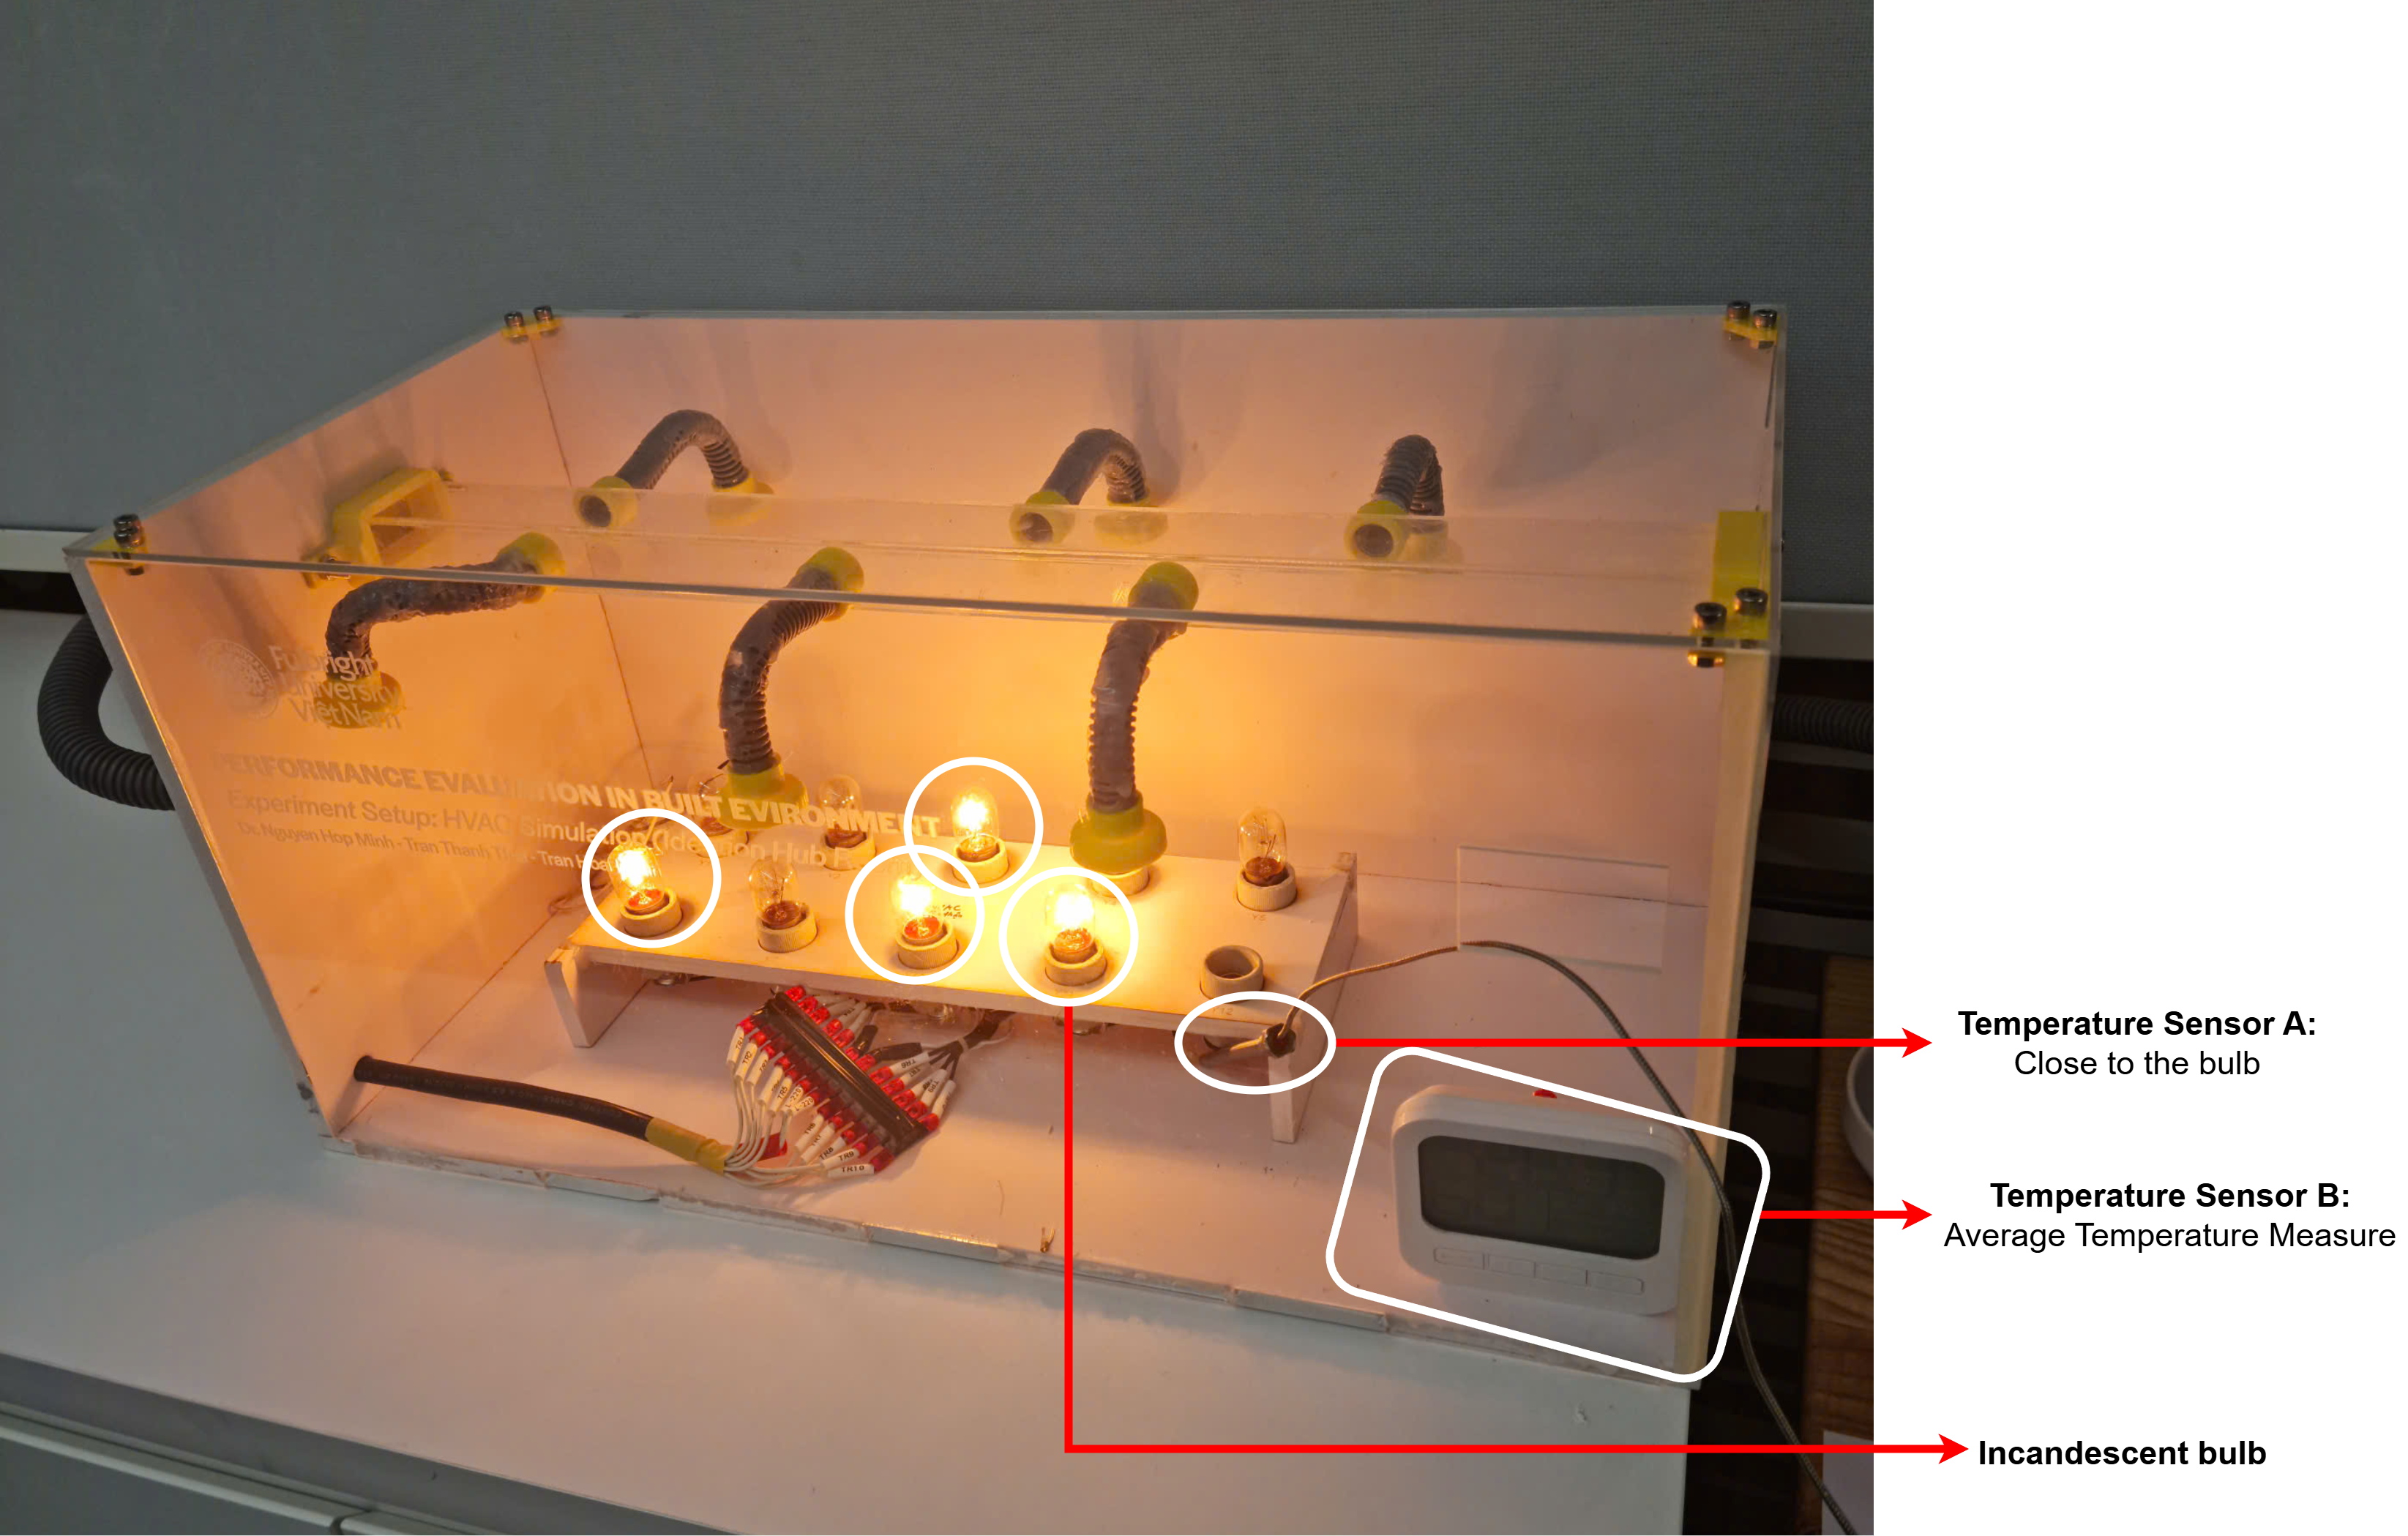
\includegraphics[width=0.85\linewidth]{SensorPlacement.png}
\end{center}

\vspace{0.15em}
Hot bulb (center), Sensor A close ($d_A$), Sensor B farther ($d_B$). Heat diffuses with decreasing intensity.
}

\block{4. Kalman Filter Solution}{
\textbf{Probabilistic Framework:} Bayesian inference with Gaussian distributions.

\vspace{0.15em}
\textbf{Prior belief:} $p(x) = \mathcal{N}(x; \hat{x}, P)$ where $x = T_{\text{bulb}}$ is hidden state.

\textbf{Likelihood:} $p(z|x) = \mathcal{N}(z; Hx, R)$ where $z$ = sensor measurement.

\textbf{Posterior:} By Bayes' rule, $p(x|z) \propto p(z|x) \cdot p(x)$ yields:
\begin{equation*}
p(x|z) = \mathcal{N}(x; \mu_{\text{post}}, \sigma^2_{\text{post}})
\end{equation*}

The Kalman Filter computes $\mu_{\text{post}}$ and $\sigma^2_{\text{post}}$ in closed form:

\vspace{0.2em}
\innerblock[]{Prediction Step (Prior Propagation)}{
\begin{align*}
\hat{x}_{\text{pred}} &= \hat{x}_{\text{prev}} \quad \text{(propagate mean)} \\
P_{\text{pred}} &= P_{\text{prev}} + Q \quad \text{(increase uncertainty)}
\end{align*}
This gives prior $p(x) = \mathcal{N}(x; \hat{x}_{\text{pred}}, P_{\text{pred}})$ before measurement.
}

\vspace{0.15em}
\innerblock[]{Update Step (Posterior via Bayes)}{
\textbf{Sensor A:} Combine prior with likelihood $p(z_A|x) = \mathcal{N}(z_A; H_A x, R_A)$
\begin{align*}
K_A &= \frac{P_{\text{pred}}}{P_{\text{pred}} + R_A} \quad \text{(Bayes weight)} \\
\hat{x}_A &= \hat{x}_{\text{pred}} + K_A(z_A - H_A\hat{x}_{\text{pred}}) \quad \text{(posterior mean)} \\
P_A &= (1 - K_A H_A) P_{\text{pred}} \quad \text{(posterior variance)}
\end{align*}

\textbf{Sensor B:} Update again with $p(z_B|x) = \mathcal{N}(z_B; H_B x, R_B)$
\begin{align*}
K_B &= \frac{P_A}{P_A + R_B}, \quad
\hat{x}_{\text{new}} = \hat{x}_A + K_B(z_B - H_B\hat{x}_A), \quad
P_{\text{new}} = (1 - K_B H_B) P_A
\end{align*}
}
}

%==============================================================================
% RIGHT COLUMN (Larger)
%==============================================================================
\column{0.34}

\block{Real Experimental Data}{
\centering
\includegraphics[width=0.95\linewidth]{experimental_results.png}

\vspace{0.2em}
\small
\textbf{Setup:} Heat source box, two ambient sensors
\begin{itemize}[leftmargin=*,itemsep=0.03em]
  \item $d_A = 5$cm (close), $d_B = 15$cm (far)
  \item $R_A = 2.0$ (noisier), $R_B = 0.5$ (stable)
  \item Process noise: $Q = 0.1$
\end{itemize}

\vspace{0.2em}
\textbf{Key Results at $t=100$s:}
\begin{itemize}[leftmargin=*,itemsep=0.03em]
  \item Sensor A: 40.5°C (close, noisy)
  \item Sensor B: 31.5°C (far, stable)
  \item \textbf{KF bulb estimate: 69.0°C}
\end{itemize}

\vspace{0.2em}
\textbf{Overall Statistics (600s):}
\begin{itemize}[leftmargin=*,itemsep=0.03em]
  \item Sensor A: Mean=36.4°C, Std=2.1°C
  \item Sensor B: Mean=30.5°C, Std=0.6°C
  \item Bulb estimate: Mean=67.2°C, Std=2.2°C
\end{itemize}

\vspace{0.2em}
\small
Data from Dr. Nguyen Hop Minh's Building Environment Performance Evaluation box.
}

\block{5. Discussion}{
\textbf{Method Overview:}
\begin{itemize}[leftmargin=*,itemsep=0.03em]
    \item \textbf{Challenge:} Estimate hidden bulb temperature from indirect air sensor measurements
    \item \textbf{Approach:} Sequential Bayesian inference via Kalman Filter with two complementary sensors
\end{itemize}

\vspace{0.2em}
\textbf{Experimental Results:}
\begin{itemize}[leftmargin=*,itemsep=0.03em]
    \item Bulb estimate: Mean=67.2°C, Std=2.2°C (600s)
    \item KF fuses Sensor A (close, noisy) with Sensor B (far, stable)
    \item Kalman Gain adaptively weights sensors by uncertainty
\end{itemize}

\vspace{0.2em}
\textbf{Interactive Demo:}\\
\url{https://leonathn.github.io/FinalProjectProbability}
}

\block{6. References}{
\footnotesize
[1] Kalman (1960). \textit{J. Basic Eng.} [2] Welch \& Bishop (2006). \textit{UNC.} [3] Simon (2006). \textit{Wiley.}
}

\end{columns}

\end{document}
